% !TEX root = main.tex
\section{課題}

\subsection*{課題1:XAMPPのインストールと起動確認}

本課題では,XAMPPのインストールおよびApacheの起動確認を行う.
この作業は実験Ⅰにて完了済みであるため,ここでは割愛する.

\subsection*{課題2:新しいデータベースの作成と表示の修正}

\subsubsection*{1. year\_of\_birth テーブルの追加}

既存の \texttt{name} および \texttt{birthplace} テーブルに加えて,新たに \texttt{year\_of\_birth} テーブルを作成し,生年情報を管理する.

\begin{figure}[htbp]
    \centering
    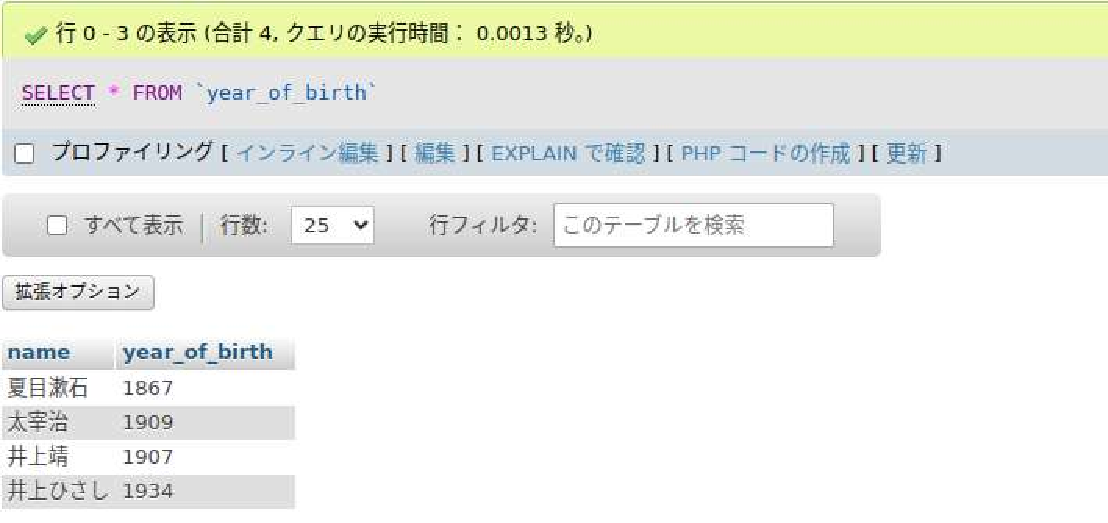
\includegraphics[width=0.9\linewidth]{figure/5.pdf}
    \caption{\texttt{maizuru} のyear\_of\_birthテーブル}
\end{figure}

\subsubsection*{2. PHPコードの修正}

3つのテーブル \texttt{name},\texttt{birthplace},\texttt{year\_of\_birth} を結合し,生年情報も含めて表示するように \texttt{select.php} を修正した.

\begin{lstlisting}[language=php]
<html>
<head>
<meta http-equiv="Content-Type" content="text/html; charset=utf-8" />
<title>PHP TEST</title>
</head>
<body>
<?php
$link = mysqli_connect('localhost', 'root', 'password');
if (!$link) {
    die('接続失敗です。'.mysql_error());
}
print('<p>接続に成功しました。</p>');

$db_selected = mysqli_select_db($link,'maizuru');
if (!$db_selected){
    die('データベース選択失敗です。'.mysql_error());
}
print('<p>データベースを選択しました。</p>');

mysqli_set_charset($link,'utf8');

$result = mysqli_query($link,'SELECT name.no, name.name, birthplace.birthplace, year_of_birth.year_of_birth FROM name INNER JOIN birthplace ON name.name = birthplace.name INNER JOIN year_of_birth ON name.name = year_of_birth.name');
if (!$result) {
    die('クエリーが失敗しました。'.mysqli_error());
}

while ($row = mysqli_fetch_assoc($result)) {
    print('<p>');
    print('id='.$row['no']);
    print(', name='.$row['name']);
    print(', birthplace='.$row['birthplace']);
    print(', year_of_birth='.$row['year_of_birth']);
    print('</p>');
}

$close_flag = mysqli_close($link);
if ($close_flag){
    print('<p>切断に成功しました。</p>');
}
?>
</body>
</html>
\end{lstlisting}

これにより,新たに生年情報を含めたWebデータベースの表示が可能となった.

\subsection*{課題3:Google Maps APIを用いたWebデータベースの作成}

\subsubsection*{1. markersテーブルへの登録}

新たに6件の舞鶴市内の飲食店情報を登録した.

\begin{lstlisting}[language=SQL]
INSERT INTO `markers` (`id`, `name`, `address`, `lat`, `lng`, `type`) VALUES
('1', 'Dairokumaru', '580 Darling Street, Rozelle, NSW', '35.4490856', '135.3105046', 'seafood'),
('2', 'Maikei Kamiagu', '76 Wilford Street, Newtown, NSW', '35.4508761', '135.3312693', 'seafood'),
('3', 'Kirameki no Tori', '36 Blue St, North Sydney NSW', '35.4806006', '135.4229714', 'ramen'),
('4', 'NetsuretsuRamen', '2 Huntley Street, Alexandria, NSW', '35.4809550', '135.4257069', 'ramen'),
('5', 'Manma frypan', '43 Macpherson Street, Bronte, NSW', '35.4671916', '135.3943122', 'cafe'),
('6', 'cafe de BONO', '60-64 Reservoir Street, Surry Hills, NSW', '35.4761566', '135.3901868', 'cafe');
\end{lstlisting}

\subsubsection*{2. 地図初期位置の変更}

舞鶴市中心の座標に地図の初期表示位置を設定するよう,JavaScript関数 \texttt{initAutocomplete()} を修正した.

\begin{lstlisting}[language=javascript]
function initAutocomplete() {
  // 地図の初期設定
  map = new google.maps.Map(document.getElementById("map"), {
    center: { lat: 35.4761566, lng: 135.3901868 }, // 舞鶴の中心
    zoom: 13, // 初期ズームレベル
    mapTypeId: "roadmap",
  });
}
\end{lstlisting}

これにより,舞鶴市の飲食店情報を視覚的に確認できるWeb地図アプリケーションが実現した.
